% A LaTeX (non-official) template for ISAE projects reports
% Copyright (C) 2014 Damien Roque
% Version: 0.2
% Author: Damien Roque <damien.roque_AT_isae.fr>

\documentclass[a4paper,12pt]{book}
\usepackage[utf8]{inputenc}
\usepackage[T1]{fontenc}
%\usepackage[frenchb]{babel} % If you write in French
\usepackage[english]{babel} % If you write in English
\usepackage{a4wide}
\usepackage{graphicx}
\graphicspath{{images/}}
\usepackage{subfig}
\usepackage{tikz}
\usetikzlibrary{shapes,arrows}
\usepackage{pgfplots}
\pgfplotsset{compat=newest}
\pgfplotsset{plot coordinates/math parser=false}
\newlength\figureheight
\newlength\figurewidth
\pgfkeys{/pgf/number format/.cd,
set decimal separator={,\!},
1000 sep={\,},
}
\usepackage{ifthen}
\usepackage{ifpdf}
\ifpdf
\usepackage[pdftex]{hyperref}
\else
\usepackage{hyperref}
\fi
\usepackage{color}
\hypersetup{%
colorlinks=true,
linkcolor=black,
citecolor=black,
urlcolor=black}

\renewcommand{\baselinestretch}{1.05}
\usepackage{fancyhdr}
\pagestyle{fancy}
\fancyfoot{}
\fancyhead[LE,RO]{\bfseries\thepage}
\fancyhead[RE]{\bfseries\nouppercase{\leftmark}}
\fancyhead[LO]{\bfseries\nouppercase{\rightmark}}
\setlength{\headheight}{15pt}

\let\headruleORIG\headrule
\renewcommand{\headrule}{\color{black} \headruleORIG}
\renewcommand{\headrulewidth}{1.0pt}
\usepackage{colortbl}
\arrayrulecolor{black}

\fancypagestyle{plain}{
  \fancyhead{}
  \fancyfoot[C]{\thepage}
  \renewcommand{\headrulewidth}{0pt}
}

\makeatletter
\def\@textbottom{\vskip \z@ \@plus 1pt}
\let\@texttop\relax
\makeatother

\makeatletter
\def\cleardoublepage{\clearpage\if@twoside \ifodd\c@page\else%
  \hbox{}%
  \thispagestyle{empty}%
  \newpage%
  \if@twocolumn\hbox{}\newpage\fi\fi\fi}
\makeatother

\usepackage{amsthm}
\usepackage{amssymb,amsmath,bbm}
\usepackage{array}
\usepackage{bm}
\usepackage{multirow}
\usepackage[footnote]{acronym}
\usepackage{float}
\usepackage{amsmath}
\usepackage{array}
\newcolumntype{L}[1]{>{\raggedright\let\newline\\\arraybackslash\hspace{0pt}}m{#1}}
\newcolumntype{C}[1]{>{\centering\let\newline\\\arraybackslash\hspace{0pt}}m{#1}}
\newcolumntype{R}[1]{>{\raggedleft\let\newline\\\arraybackslash\hspace{0pt}}m{#1}}



\newcommand*{\SET}[1]  {\ensuremath{\mathbf{#1}}}
\newcommand*{\VEC}[1]  {\ensuremath{\boldsymbol{#1}}}
\newcommand*{\FAM}[1]  {\ensuremath{\boldsymbol{#1}}}
\newcommand*{\MAT}[1]  {\ensuremath{\boldsymbol{#1}}}
\newcommand*{\OP}[1]  {\ensuremath{\mathrm{#1}}}
\newcommand*{\NORM}[1]  {\ensuremath{\left\|#1\right\|}}
\newcommand*{\DPR}[2]  {\ensuremath{\left \langle #1,#2 \right \rangle}}
\newcommand*{\calbf}[1]  {\ensuremath{\boldsymbol{\mathcal{#1}}}}
\newcommand*{\shift}[1]  {\ensuremath{\boldsymbol{#1}}}

\newcommand{\eqdef}{\stackrel{\mathrm{def}}{=}}
\newcommand{\argmax}{\operatornamewithlimits{argmax}}
\newcommand{\argmin}{\operatornamewithlimits{argmin}}
\newcommand{\ud}{\, \mathrm{d}}
\newcommand{\vect}{\text{Vect}}
\newcommand{\sinc}{\ensuremath{\mathrm{sinc}}}
\newcommand{\esp}{\ensuremath{\mathbb{E}}}
\newcommand{\hilbert}{\ensuremath{\mathcal{H}}}
\newcommand{\fourier}{\ensuremath{\mathcal{F}}}
\newcommand{\sgn}{\text{sgn}}
\newcommand{\intTT}{\int_{-T}^{T}}
\newcommand{\intT}{\int_{-\frac{T}{2}}^{\frac{T}{2}}}
\newcommand{\intinf}{\int_{-\infty}^{+\infty}}
\newcommand{\Sh}{\ensuremath{\boldsymbol{S}}}
\newcommand{\C}{\SET{C}}
\newcommand{\R}{\SET{R}}
\newcommand{\Z}{\SET{Z}}
\newcommand{\N}{\SET{N}}
\newcommand{\K}{\SET{K}}
\newcommand{\reel}{\mathcal{R}}
\newcommand{\imag}{\mathcal{I}}
\newcommand{\cmnr}{c_{m,n}^\reel}
\newcommand{\cmni}{c_{m,n}^\imag}
\newcommand{\cnr}{c_{n}^\reel}
\newcommand{\cni}{c_{n}^\imag}
\newcommand{\tproto}{g}
\newcommand{\rproto}{\check{g}}
\newcommand{\LR}{\mathcal{L}_2(\SET{R})}
\newcommand{\LZ}{\ell_2(\SET{Z})}
\newcommand{\LZI}[1]{\ell_2(\SET{#1})}
\newcommand{\LZZ}{\ell_2(\SET{Z}^2)}
\newcommand{\diag}{\operatorname{diag}}
\newcommand{\noise}{z}
\newcommand{\Noise}{Z}
\newcommand{\filtnoise}{\zeta}
\newcommand{\tp}{g}
\newcommand{\rp}{\check{g}}
\newcommand{\TP}{G}
\newcommand{\RP}{\check{G}}
\newcommand{\dmin}{d_{\mathrm{min}}}
\newcommand{\Dmin}{D_{\mathrm{min}}}
\newcommand{\Image}{\ensuremath{\text{Im}}}
\newcommand{\Span}{\ensuremath{\text{Span}}}

\newtheoremstyle{break}
  {11pt}{11pt}%
  {\itshape}{}%
  {\bfseries}{}%
  {\newline}{}%
\theoremstyle{break}

%\theoremstyle{definition}
\newtheorem{definition}{Définition}[chapter]

%\theoremstyle{definition}
\newtheorem{theoreme}{Théorème}[chapter]

%\theoremstyle{remark}
\newtheorem{remarque}{Remarque}[chapter]

%\theoremstyle{plain}
\newtheorem{propriete}{Propriété}[chapter]
\newtheorem{exemple}{Exemple}[chapter]

\parskip=5pt
%\sloppy

\usepackage{Sweave}
\begin{document}
\Sconcordance{concordance:finnn.tex:finnn.Rnw:%
1 165 1 1 0 73 1 1 29 22 1 1 8 41 1 1 43 10 1 1 7 1 2 16 1 1 14 1 2 9 1 %
1 55 1 2 5 1 1 43 1 2 4 1 1 43 1 2 5 1 1 43 1 2 9 1 1 7 4 0 1 2 12 1 1 %
19 4 1 1 3 16 0 1 16 1 2 2 1 1 9 1 2 4 1 1 9 3 0 1 8 3 0 1 2 3 1 1 20 3 %
0 1 8 2 0 1 19 2 0 1 8 2 0 1 19 2 0 1 8 2 0 1 19 2 0 1 8 2 0 1 19 2 0 1 %
8 2 0 1 19 2 0 1 8 2 0 1 19 2 0 1 8 2 0 1 19 2 0 1 8 2 0 1 19 2 0 1 8 2 %
0 1 19 2 0 1 8 3 0 1 2 11 1}


%%%%%%%%%%%%%%%%%%
%%% First page %%%
%%%%%%%%%%%%%%%%%%

\begin{titlepage}
\begin{center}

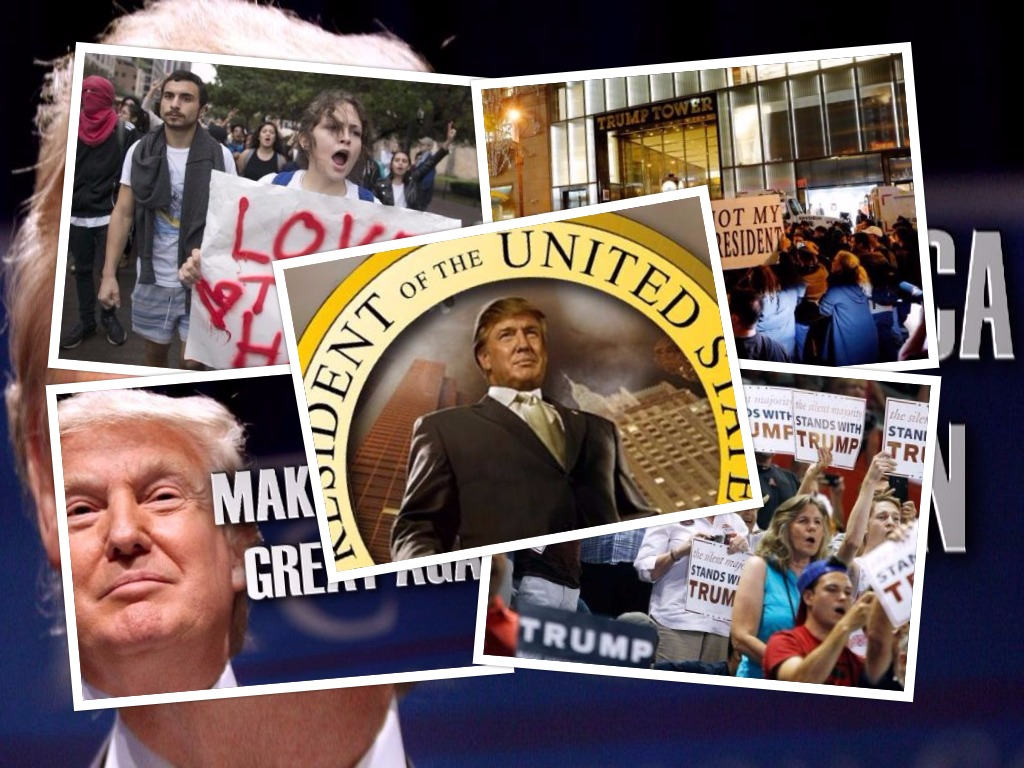
\includegraphics[width=0.6\textwidth]{logo}\\[1cm]

{\large The Wharton School, University of Pennsylvania}\\[0.5cm]

{\large A project report on}\\[0.5cm]

% Title
\rule{\linewidth}{0.5mm} \\[0.4cm]
{ \huge \bfseries Sentiment Analysis after US elections \\[0.4cm] }
\rule{\linewidth}{0.5mm} \\[1.5cm]

% Author and supervisor
\noindent
\begin{minipage}{0.4\textwidth}
  \begin{flushleft} \large
    \emph{Author :}\\
    Rahul Dhakecha
  \end{flushleft}
\end{minipage}%
\begin{minipage}{0.4\textwidth}
  \begin{flushright} \large
    \emph{Professor :} \\
    Dr. Linda Zhao 
  \end{flushright}
\end{minipage}

\vfill

% Bottom of the page
{\large Course: STAT 571, Modern Data Mining\\ \today}

\end{center}
\end{titlepage}

%%%%%%%%%%%%%%%%%%%%%%%%%%%%%
%%% Non-significant pages %%%
%%%%%%%%%%%%%%%%%%%%%%%%%%%%%

\frontmatter

\chapter*{Summary}
“Statistics and data science gets more credit than it deserves when it’s correct—and more blame than it deserves when it’s incorrect.” - Anthony Goldbloom, CEO of Kaggle.

This statement was more than validated on November 8th 2016, witnessing mixed emotions spread throughout the country, with few people being extremely happy while others deeply disheartened. But the most serious blow was to the statisticians and data science community. We know Data Science went wrong in the 2016 US elections. Well, it was a prediction and predictions might go wrong. Should we cease to rely on such techniques? Should we stop relying on weather forecasts and other such crucial applications of learning and data science? Ofcourse, we know the answer. Data science banks on tons of assumptions, few being extremely naive. These assumptions may sometimes come out completely wrong, which eventually leads to the failure of data science. Nevertheless, data science is competent enough to give the gist of the happenings around the world.

In this report, we analyze the sentiments of people for our president elect Donald Trump. This report is mainly divided into two parts. First part analyzes the variation in sentiments of people over a period of past one month, from November 8th to December 8th 2016. Second part focuses on more recent sentiments of people, from December 10th to December 17th 2016. Second part is further broken down to analyze common sentiments over different states of the US.

\clearpage
\tableofcontents

\clearpage
\listoffigures

\clearpage

%%%%%%%%%%%%%%%%%%%%%%%%%%%%%%%%%%%%%%%%%%%%
%%% Content of the report and references %%%
%%%%%%%%%%%%%%%%%%%%%%%%%%%%%%%%%%%%%%%%%%%%

\mainmatter
\pagestyle{fancy}

\cleardoublepage





\chapter{Part I}

As mentioned earlier, first part of analysis focuses on the variation of sentiments across one month. For the purpose of sentiment analysis, data is downloaded from Twitter, one of the largest microblogging site in terms of users. 

\section{Data Acquisition}

Twitter API provides an easy access for tweets to be downloaded on R platform. But this access is limited to the tweets from past one week only. It becomes a non trivial task to access a month old tweets. Packages like rvest in R are very handy to scrap through online content but owing to the flexibility and availability of Python repositories, Twitter data in this part of the report is accessed with the help of Python. 

Github repository[link here] was modified to access the specific contents for this report. Tweets were filtered based on the keyword and time frame. Tweeets were encoded using utf-8 encoding which is compatible with R. Further these tweets were saved as new line separated content in a single text file. Following snapshot provides the commands used for the above mentioned steps.

\begin{figure}[H]
\centering
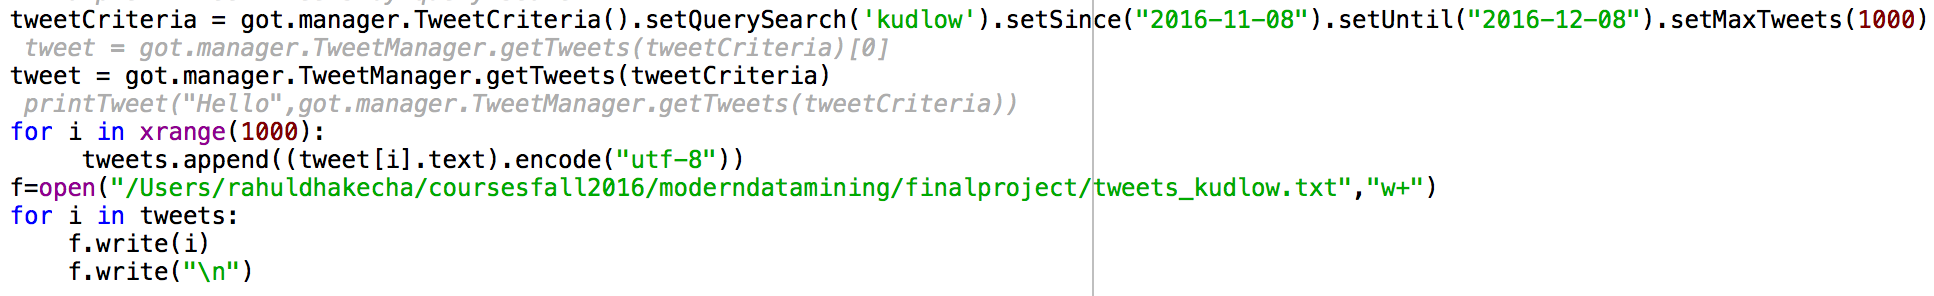
\includegraphics[scale=1.0]{snapshot1.png}
\caption{Python code}
\label{fig:2}
\end{figure}

In the above code snippet, 1000 tweets from November 8th 2016 to December 8th 2016 which contains the keyword $"kudlow"$ is accessed and stored in a text file named $"text\_kudlow"$, with new line character separating each tweet. This text file is then directly accessed through R code.


In the similar fashion, we develop five different files summarized in following table.

\begin{center}
\begin{tabular}{ |C{1.9cm}|C{1.9cm}|C{1.9cm}|C{1.9cm}|C{1.9cm}|C{1.9cm}| } 
 \hline
 File name & Description & Keyword & Since & Until & number \\ 
 \hline
 data\_tweets \_08\_Nov & for sentiment analysis immediately after election & trump & 11/08/2016 & 11/16/2016 & 5000 \\
 \hline
 data\_tweets \_01\_Dec & for sentiment analysis after one month of election & trump & 12/01/2016 & 12/08/2016 & 5000 \\
  \hline
 data\_tweets \_obama \_speech & for sentiment analysis after Obama's speech & obama speech & 11/08/2016 & 12/08/2016 & 1000 \\
  \hline
 data\_tweets \_bannon & after nomination of Bannon & bannon & 11/08/2016 & 12/08/2016 & 1000 \\
  \hline
 data\_tweets \_kudlow & after nomination of Kudlow & kudlow & 11/08/2016 & 12/08/2016 & 1000 \\
 \hline
\end{tabular}
\end{center}


Since this sample, in any significant way, does not represent the true population of the US, limitations of this analysis is addressed in the concluding remarks. Files obatained above are raw tweets obtained from Twitter and they need to be cleaned before using it for sentiment analysis.


\section{Data Cleaning}

Tweets obtained in raw format has variety of contents such as punctuations, url, etc which does not contribute to any significant sentiment and thus it needs to be removed. Also, we need to remove few essential elements like emojis, numbers, etc; which may contribute to the sentiment analysis but for simplicity we drop its usage.

Following steps are followed to clean the data and bring it into analyzable form.
\begin{itemize}
\item Data obtained from the text file is accessed in the form of table content and is needed to be converted into character strings. 
\item This list is then converted into corpus, which contains two parts- character string and metadata.
\item Majority of tweets have URL attached to them, which are removed as they do not contribute any significant information in sentiment analysis.
\item Many tweets are addressed to someone and this information is redundant in analysis; therefore all target elements are removed.
\item For simplicity, effect of emoticons(emojis) in this analysis is not considered. All emojis are converted into hex codes, which are removed. This assumption is one of the naive assumption as emojis convey a lot of information about the sentiment of a tweet. 
\item Entire text is converted into lower case, eliminated english stopwords, punctuations and number. Removal of english stop words like "not","nor" and "no" is again a naive step as these words convey critical information about sentiment of a particular treat. For example, a sentence like "People are not happy" is a negative statement but it will be classified as a positive sentiment after removal of english stopwords.
\item When a tweet text file is created using a particular keyword, the appearance of that keyword is gauranteed in all the tweets. Such words are removed which inspite of occuring frequently does not carry any significant amount of information.
\item Finally all the words are stemmed to retain their significance, and at the same time dropped of the extra content of the word.
\end{itemize}



After following the above mentioned steps we store the cleaned version of tweets as a plain text document in $corpus\_elect\_result$. This variable temporarily holds data for all the different text files mentioned in the section above.

\section{Analysis}
\subsection{Wordcloud}

Data rendered after data cleaning contains all significant words. To get the gist of frequently occuirng words in the tweets, a word cloud is plotted. This word cloud is obtained from $data\_tweets\_08\_Nov$.txt file.

\begin{figure}[H]
\centering

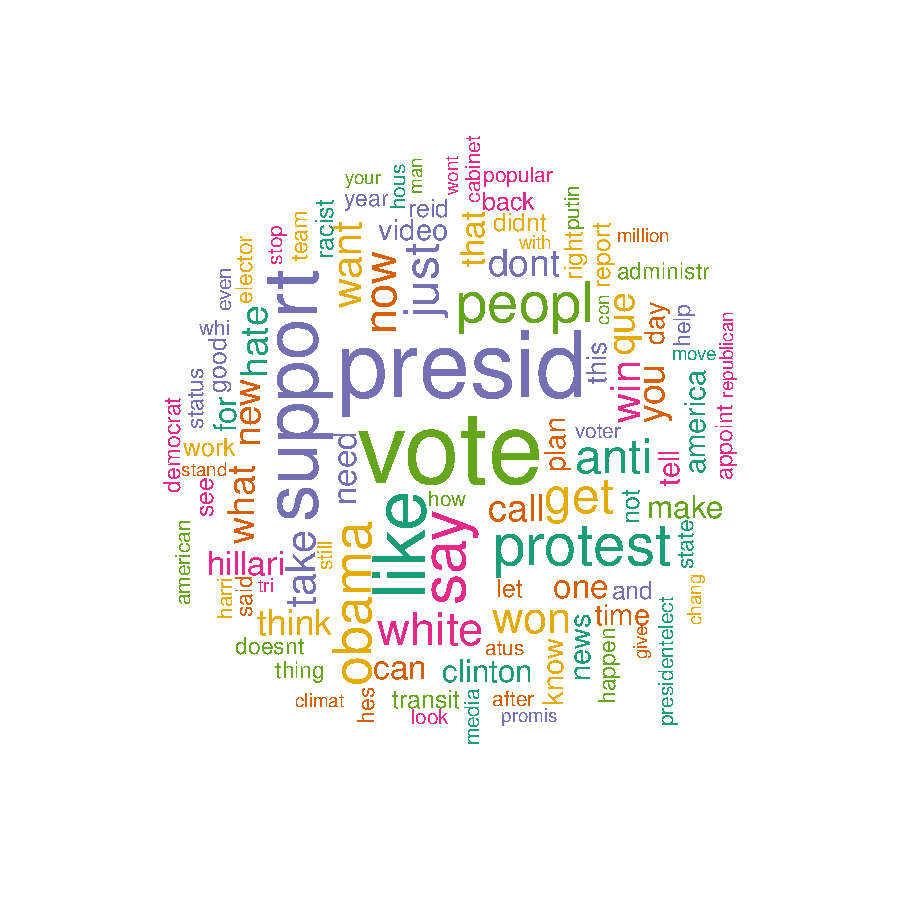
\includegraphics{finnn-r4}
\caption{Wordcloud for }
\label{fig:1}
\end{figure}

This word cloud pretty much reflects the sentiments of people during the week following the results of election. While few states were fully supporting the Republican elect Donald Trump, states like California and New York had protests for number of days. Presence of words like "support","like", "for win", etc clearly displays strong favor for the president elect while words like "protest", "hate", "racist", etc clearly shows strong disagreement of people for the results of US elections.

\subsection{Sentiments immediately after US elections}

To further dive into the text corpus, we try to segregate our analysis based on various sentiments like trust, anger, joy, etc. This analysis is carried out with the help of "syuzhet" package developed by Stanford NLP team. It implements Saif Mohammad’s NRC Emotion lexicon. According to Mohammad, “the NRC emotion lexicon is a list of words and their associations with eight emotions (anger, fear, anticipation, trust, surprise, sadness, joy, and disgust) and two sentiments (negative and positive). 



For the sake of visual clearity, we represent negative sentiment by red color and positive sentiment by green color. We divide all the words in the corpus into different sentiment categories and the resultant proportion is plotted on bar graph. The plot reveals that immediately after the results, majority of population was gripped in the wave of fear. Owing to the president elect's bold statements against minorities, Muslims and women, this fear was more than obvious. Large chunks of population came out on streets to express their griefs and anger. But at the same time, there was major proportion of population which expressed their trust on the president elect. This trust owed to the promises made by Republican candidate on creating new jobs and his ability to drive profitable businesses. Overall it can be seen that negative sentiments surpassed positive sentiments during the period following immediately after election results.


\begin{figure}[!]
\centering
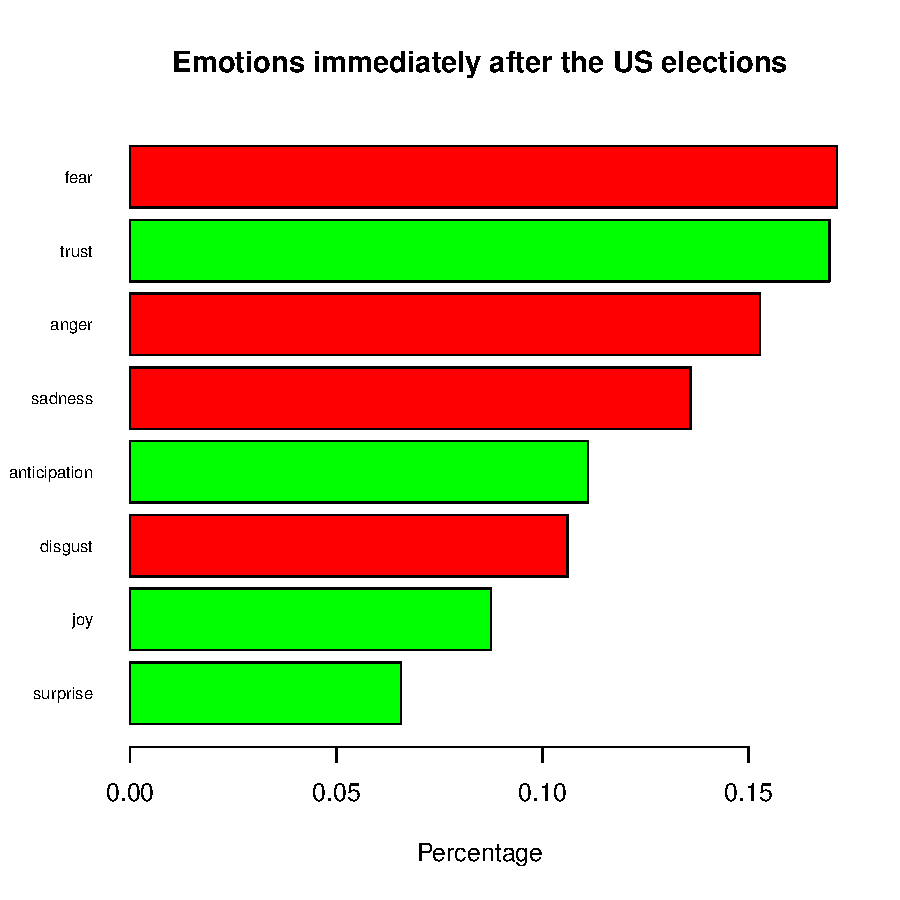
\includegraphics{finnn-r5}
\caption{Loss functions}
\label{fig:1}
\end{figure}


\subsection{Sentiments one month past US elections}
It can be seen that over the period of one month, "trust" has replaced "fear" as the maximum proportionate sentiment among people. Nevertheless, this change is not significant by a huge margin. But it definitely shows that people are coming in support for new government irrespective of the differences in their thoughts and philosophy. 



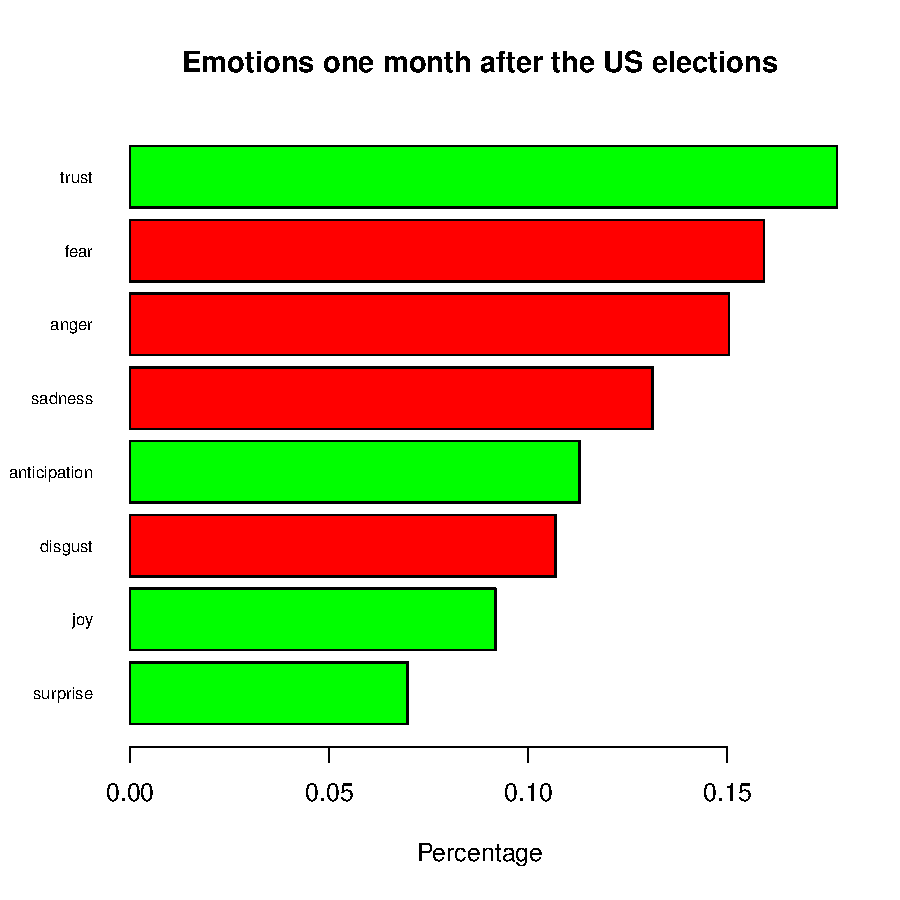
\includegraphics{finnn-r6}


Also, it can be seen that there is still around 30 percent of people expressing sadness and anger in some or the other way. One month after the results has witnessed several major and minor events which has swayed people's emotions. We take a look at few of the prominent ones and try to reflect the sentiments based on the word cloud.

\subsection{Sentiments after Obama's speech over President elect}

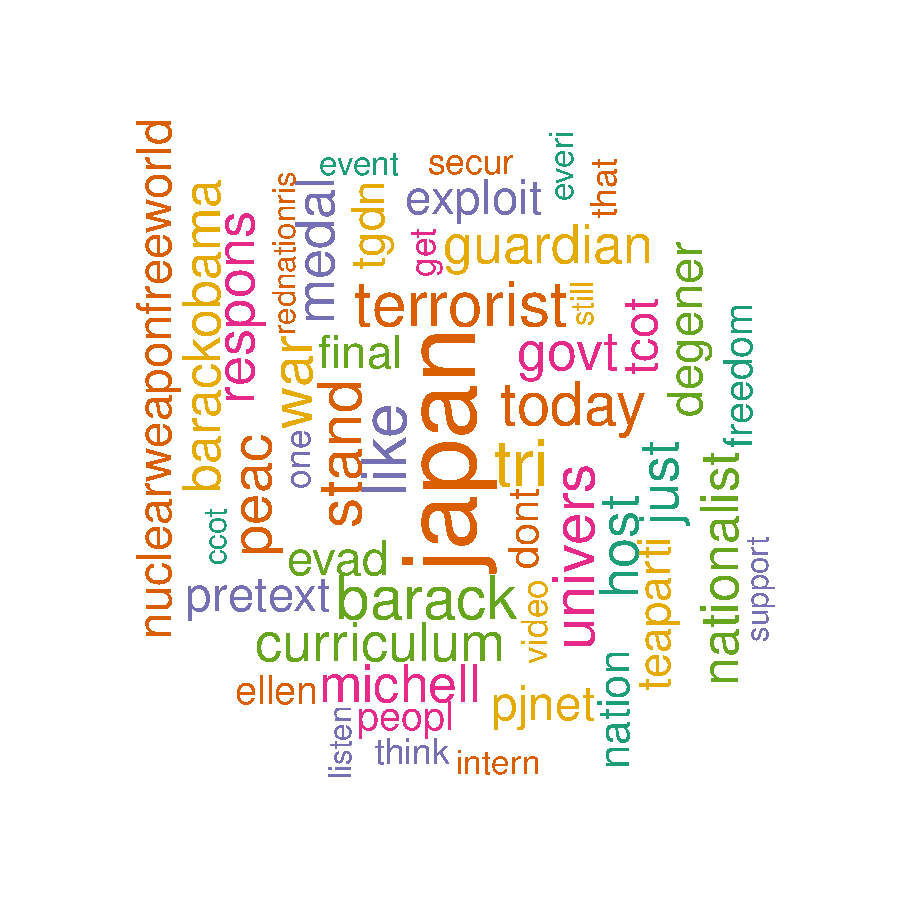
\includegraphics{finnn-r7}

Despite strong differences in opinions on matter of sheer importance, current president Barack Obama gave congratulatory speech on Novemeber 9th at White House. This speech addressed the positivies of the new government and was in the direction of soothing the angry mob. He assured smooth transition of government and assured befitting atmosphere for the coming generations. Enhancing the spirit of patriotism, this speech definitely wooed the mass.

\subsection{Sentiments after appointment of Steve Bannon as chief White House strategist}

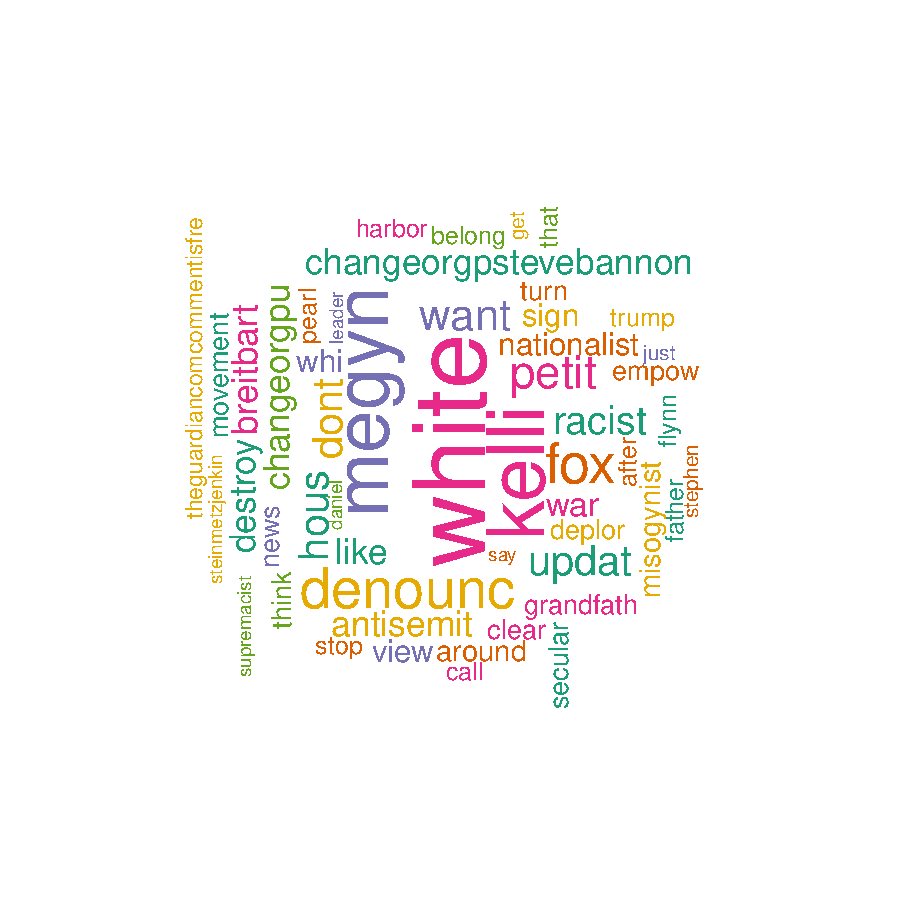
\includegraphics{finnn-r8}

Steve Bannon was CEO of Donald Trump's presidential campaign and was later appointed as Chief Strategist at White House on November 13th 2016. This appointment saw severe opposition from many groups especially from Anti Defamation League and Council on American Islamic relations. Bannon is often considered racist, white nationalist and anti Semitic. Words like "white", "antisemit", "racist", etc portray this polarity in Bannon's view. Words like "stop","don't", etc displays negative public opinion towards this appointment.


\subsection{Sentiments after appointment of Larry Kudlow as Chairman of Council of Economic Advisor}

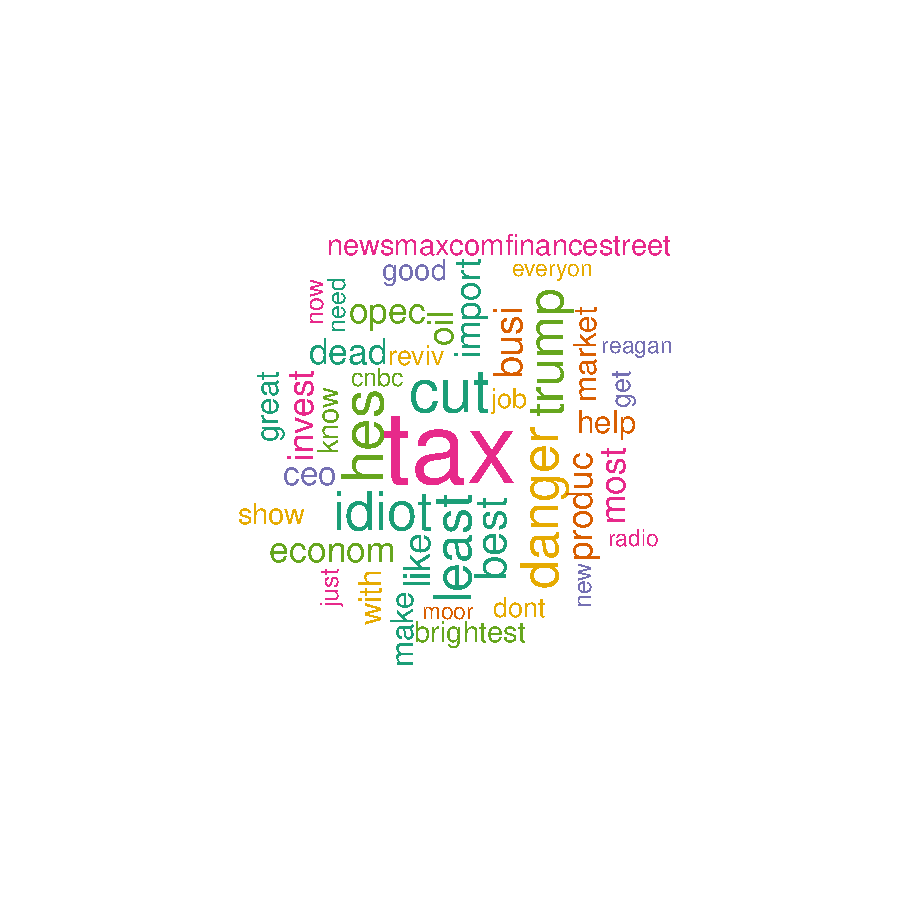
\includegraphics{finnn-r9}

Another major decision which raised eyes was president elect's nomination of Larry Kudlow as Chairman of Council of Economic Advisor. While Kudlow does not have controversies following him as Steve Bannon, but his academic inexperience leaves many loop holes to be filled. Position which was once chaired by great economists such as Janet Yellen, Ben Bernanke and Alan Greenspan demands a lot of intellect and decisive power. Words like "idiot", "danger", etc reflects a sense of doubt in public.

\chapter{Part II}
In this part we directly access the data from Twitter API without involving Python. We set authorization with twitter and save the accessed data.

\section{Data Acquisition}

We download the twitter data for 10 prominent states of the US in terms of population and economy. We also pay special attention to the swing states Michigan, Pennsylvania, Florida, Ohio, Iowa, North Carolina and Wisconsin which were the deciding states in 2016 US elections. For each state, we take its capital, feed its geographical information in twitter and get 1000 tweets within a radius of 100 miles. 

\begin{Schunk}
\begin{Soutput}
[1] "Using direct authentication"
\end{Soutput}
\end{Schunk}

\section{Analysis}

\subsection{New York sentiment}

In this part, we list all positive words along with their corresponding counts. For this analysis we use "tidytext" package which gives us further flexibility to handle text data. Inherent structure of this package allows us to create different groups of sentiments. This package handles sentiments with the help of three lexicons:
\begin{itemize}
\item AFFIN - This lexicon rates different words on the scale of -5 to +5, where more negative score representing negative sentiments and vice versa.
\item Bing - This lexicon divides all the words into either positive or negative.
\item nrc - This package divides all the words into 8 different sentiments, similar to that of "syuzhet" package.
\end{itemize}
Using bing lexicon, we create bar graph representing different positive and negative sentiments.


\subsection{Positive Negative Words}

This section segregates positive and negative words from the tweet data set.

\begin{Schunk}
\begin{Soutput}
# A tibble: 2,024 × 2
             word     n
            <chr> <int>
1          #trump   925
2    @dumptrump22   217
3             lie   137
4           #maga   131
5           trump   125
6           https   122
7            hope    83
8            life    78
9     #truepundit    77
10 @trumpsuperpac    74
# ... with 2,014 more rows
\end{Soutput}
\end{Schunk}

\subsection{Wordcloud positive negative words}

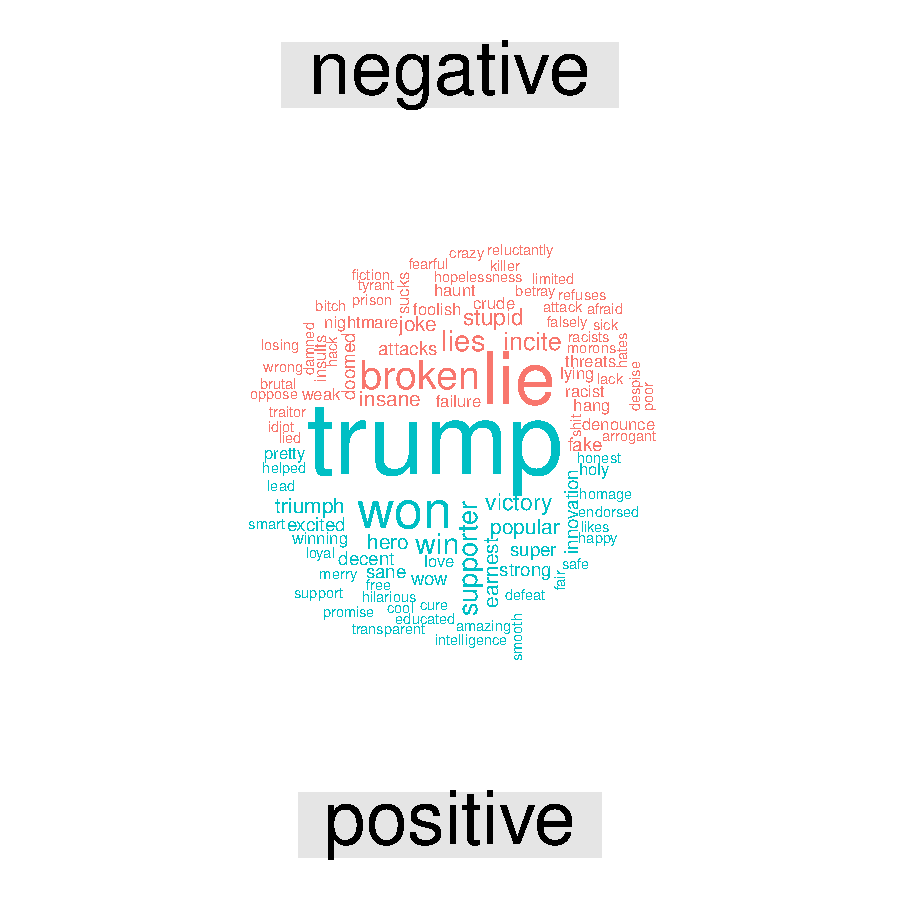
\includegraphics{finnn-r13}

\subsection{Positive Negative Words}

Finally we count total number of negative and positive words in New York state. We see that bing lexicon has total of 4782 negative words and 2006 positive words. Therefore, number of negative count will always be greater than positive count. To mitigate this effect, we will multiply the negative count by a factor of 2006/4782. This multiplication will scale down negative counts to the level of positive counts.

\begin{Schunk}
\begin{Soutput}
[1] 505
\end{Soutput}
\begin{Soutput}
[1] 338
\end{Soutput}
\end{Schunk}


In similar fashion, we analyse positive and negative word counts for different states and we find overall shift towards positive sentiments, which validates our conclusion of part I.

\begin{Schunk}
\begin{Soutput}
[1] 503
\end{Soutput}
\begin{Soutput}
[1] 287
\end{Soutput}
\begin{Soutput}
[1] 161
\end{Soutput}
\begin{Soutput}
[1] 170
\end{Soutput}
\begin{Soutput}
[1] 164
\end{Soutput}
\begin{Soutput}
[1] 98
\end{Soutput}
\begin{Soutput}
[1] 496
\end{Soutput}
\begin{Soutput}
[1] 336
\end{Soutput}
\begin{Soutput}
[1] 290
\end{Soutput}
\begin{Soutput}
[1] 236
\end{Soutput}
\begin{Soutput}
[1] 304
\end{Soutput}
\begin{Soutput}
[1] 245
\end{Soutput}
\begin{Soutput}
[1] 1005
\end{Soutput}
\begin{Soutput}
[1] 134
\end{Soutput}
\begin{Soutput}
[1] 369
\end{Soutput}
\begin{Soutput}
[1] 255
\end{Soutput}
\begin{Soutput}
[1] 102
\end{Soutput}
\begin{Soutput}
[1] 59
\end{Soutput}
\begin{Soutput}
[1] 47
\end{Soutput}
\begin{Soutput}
[1] 20
\end{Soutput}
\end{Schunk}

\section*{References}
\begin{enumerate}
\item https://github.com/mayank93/Twitter-Sentiment-Analysis/tree/master/docs
\item https://cran.r-project.org/web/packages/syuzhet/syuzhet.pdf
\item https://cran.r-project.org/web/packages/tidytext/vignettes/tidytext.html
\end{enumerate}




\end{document}
